\documentclass[10pt,twocolumn]{article}
\usepackage[letterpaper,landscape,hmargin=.7in,top=.7in,bottom=.9in]{geometry}
\usepackage[utf8]{inputenc}
\usepackage{fourier}
\usepackage[T1]{fontenc}
\usepackage{graphicx}
\usepackage[hyphens]{url}
\usepackage[hidelinks]{hyperref}
\usepackage{verbatim}
\usepackage[french]{babel}
\usepackage{microtype}

%\usepackage{layout}
%\usepackage{lipsum}
%\usepackage{showframe}

\title{Devoir \no 1\thanks{STT 1700 - Introduction à la statistique - Université de Montréal - Christian \textsc{Léger}}}
\author{Julien \textsc{Hébert-Doutreloux} \and Alexandre \textsc{Pachot}}

\setcounter{tocdepth}{1}
\renewcommand \thesubsection {\alph{subsection})}
\graphicspath{ {./images/} }


\begin{document}
%\layout

\maketitle
\tableofcontents
%\lipsum



\section{Causes de mortalités en 2017 aux États-Unis}
\subsection{Les maladies cérébrovasculaires et cardiaques}
D’après le \textit{Center for Disease Control}, les maladies cérébrovasculaires et les maladies cardiaques sont respectivement la cause de 5,2~\% et de 23,0~\% des mortalités aux États-Unis en 2017. Par conséquent, il est raisonnable de croire que les maladies cérébrovasculaires et cardiaques ont été la cause d’environ 28,2~\% des mortalités aux États-Unis en 2017.


\subsection{Autres causes de mortalité}
Maladies cardiaques, cancer, accidents, maladies respiratoires, maladies cérébrovasculaires, Alzheimer, diabète et influenza/pneumonies sont respectivement la cause de 23,0~\%, 21,3~\%, 6,0~\%, 5,7~\%, 5,2~\%, 4,3~\%, 3,0~\%, 2,0~\%, des mortalités aux États-Unis en 2017. Ce qui représente un total de 70,5~\%. Le pourcentage des autres causes de mortalités est de 29,5~\%.


\subsection{Diagramme à bâtons}
Le diagramme à bâtons est représenté à la figure~\ref{mortaliteBarplot}.

\begin{figure}[htbp]
	\caption{Diagramme à bâtons}
	\label{mortaliteBarplot}
	\centering
	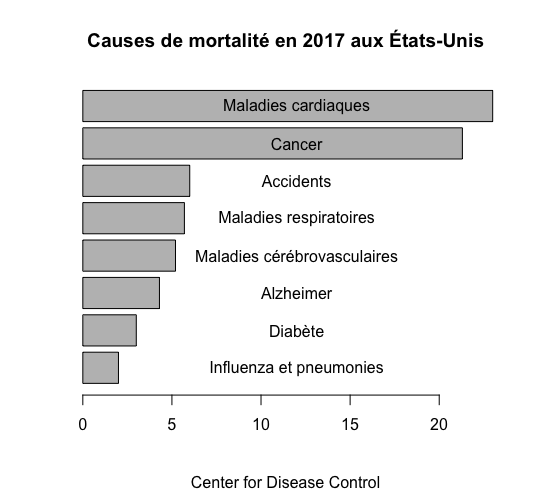
\includegraphics[width=\linewidth]{d1_mortaliteBarplot}
\end{figure}

\subsubsection*{Code R:}
\begin{verbatim}
barplot(
  c(2.0, 3.0, 4.3, 5.2, 5.7, 6.0, 21.3, 23.0),
  main = "Causes de mortalité en 2017 aux États-Unis",
  sub = "Center for Disease Control",
  horiz=TRUE)
text(x = 12, y = 9.1, labels = "Maladies cardiaques")
text(x = 12, y = 7.9, labels = "Cancer")
text(x = 12, y = 6.7, labels = "Accidents")
text(x = 12, y = 5.5, labels = "Maladies respiratoires")
text(x = 12, y = 4.3, labels = "Maladies cérébrovasculaires")
text(x = 12, y = 3.1, labels = "Alzheimer")
text(x = 12, y = 1.9, labels = "Diabète")
text(x = 12, y = .7, labels = "Influenza et pneumonies")
\end{verbatim}


\subsection{Diagramme circulaire}
Le diagramme circulaire est représenté à la figure~\ref{mortalitePie}. On remarque qu’il est plus facile de voir les petites différences entre les causes qui ont des pourcentages semblables (accidents, maladies respiratoires, maladies cérébrovasculaires et alzheimer) dans le diagramme à bâtons.

\begin{figure}[htbp]
	\caption{Diagramme circulaire}
	\label{mortalitePie}
	\centering
	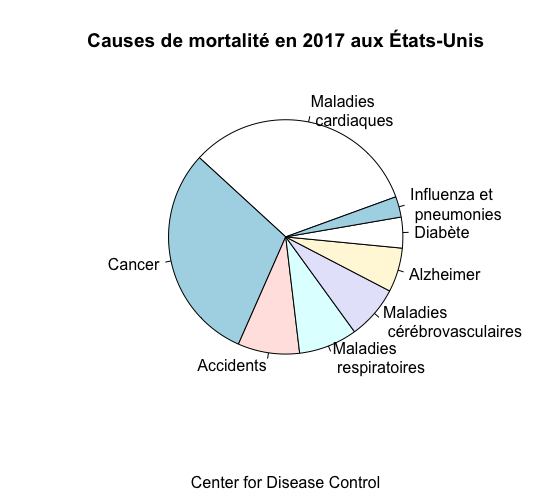
\includegraphics[width=\linewidth]{d1_mortalitePie}
\end{figure}

\subsubsection*{Code R:}
\begin{verbatim}
pie(
  c(23.0, 21.3, 6.0, 5.7, 5.2, 4.3, 3.0, 2.0),
  labels = c("Maladies\n cardiaques","Cancer","Accidents",
    "Maladies\n respiratoires","Maladies\n cérébrovasculaires",
    "Alzheimer","Diabète","Influenza et\n pneumonies"),
  main = "Causes de mortalité en 2017 aux États-Unis",
  sub = "Center for Disease Control",
  init.angle = 20)
\end{verbatim}


\subsection{Brève description}
On peut catégoriser les causes de mortalité en 2017 aux États-Unis en deux groupes. Il y a d’une part les maladies cardiaques et les cancers qui représentent chacune d’entre elles plus de 20~\% des causes de mortalité, alors que les autres causes de mortalité représentées sur ces diagrammes ne dépassent pas individuellement les 6~\%.



\section{Examen intra de la session Automne 2019}
\subsection{Diagramme à moustaches}
Sur le diagramme à moustaches (fig.~\ref{intraBoxplot}), la médiane est légèrement supérieure à 60~\% : la moitié des étudiants ont eu plus de 60~\%. Le premier quartile ($Q_{1}$) est en dessous des 50~\% : un quart des étudiants sont en échec à l’intra. Le troisième quartile ($Q_{3}$) est au-dessus de 70~\%, ce qui veut dire qu’un quart des étudiants ont eu au moins cette note-là.

\begin{figure}[htbp]
	\caption{Diagramme à moustaches}
	\label{intraBoxplot}
	\centering
	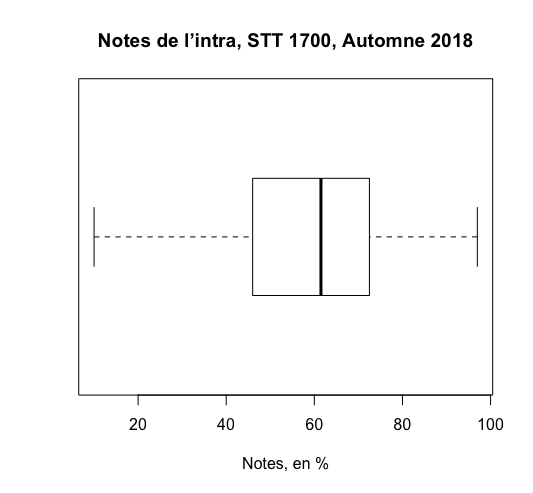
\includegraphics[width=\linewidth]{d1_intraBoxplot}
\end{figure}

Le graphique a été fait avec R, avec les paramètres par défaut. Lorsqu’il y a des \og données aberrantes\fg{}, c’est-à-dire qui dépassent une fois et demie l’écart interquartile ($EI = Q_{3} - Q_{1}$), interquartile range (IQR) en anglais, R représente ces données par des cercles. Il n’y a pas de données considérées comme aberrantes dans cette distribution. On remarque également que personne n’a eu un 100~\% ni un zéro.

\subsubsection*{Code R:}
\begin{verbatim}
intra<-read.table(file="~/d1_intra.txt")
boxplot(
  intra,
  main = "Notes de l’intra, STT 1700, Automne 2019",
  xlab = "Notes, en %",
  horizontal = TRUE)
\end{verbatim}


\subsection{Graphique quantiles normaux}
Lorsqu’on observe le graphique des quantiles normaux (fig.~\ref{intraQqnorm}), on remarque que les points sont alignés sur la première bissectrice, on peut en déduire que la distribution des notes suit une loi normale.

\begin{figure}[htbp]
	\caption{Graphique quantiles normaux}
	\label{intraQqnorm}
	\centering
	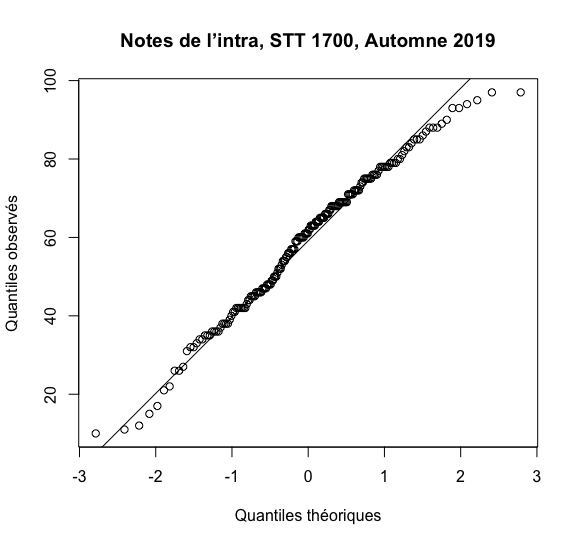
\includegraphics[width=\linewidth]{d1_intraQqnorm}
\end{figure}

\subsubsection*{Code R:}
\begin{verbatim}
qqnorm(
  intra$V1,
  main = "Notes de l’intra, STT 1700, Automne 2019",
  xlab = "Quantiles théoriques",
  ylab = "Quantiles observés")
qqline(intra$V1)
\end{verbatim}


\subsection{Histogramme}
\label{histogramme}
Lorsqu’on observe l’histogramme (fig.~\ref{intraHist}), la distribution semble bimodale. La distribution est-elle réellement bimodale ? D’après Wikipédia\footnote{\url{https://en.wikipedia.org/wiki/Multimodal\_distribution\#General\_tests}}, il existe plusieurs tests pour savoir si une distribution est unimodale. Parmi ces tests, il y a le Hartigan’s dip statistic (HDS) test qui peut se faire sous R à partir de l’extension \textit{diptest} (Hartigan's Dip Test Statistic for Unimodality). D’après Freeman \cite{Freeman:2013aa}, une valeur inférieure à 0,05 au test HDS indique une bimodalité signicative. La valeur obtenue pour cette distribution est de 0,026. On peut considérer la distribution comme bimodale.

%https://stats.stackexchange.com/questions/156808/interpretation-of-hartigans-dip-test

\begin{figure}[htbp]
	\caption{Histogramme}
	\label{intraHist}
	\centering
	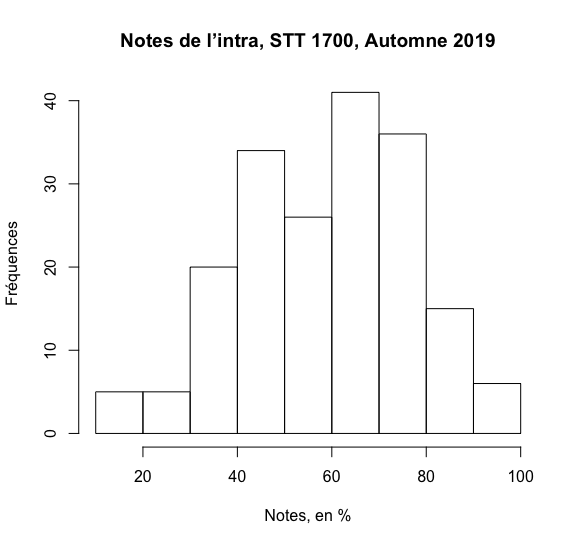
\includegraphics[width=\linewidth]{d1_intraHist}
\end{figure}

\subsubsection*{Code R:}
\begin{verbatim}
> hist(
    intra$V1,
    main = "Notes de l’intra, STT 1700, Automne 2019",
    xlab = "Notes, en %",
    ylab = "Fréquences")
> install.packages("diptest")
> require("diptest")
> dip(intra$V1)
[1] 0.02581352
\end{verbatim}


\subsection{Meilleur graphique}
Il n’y a pas de meilleur graphique, chaque graphique a ses propres caractéristiques ainsi que les avantages qui vont avec. Si je devais comparer les notes du cours de STT~1700 d’une dizaine de sessions, les diagrammes à moustaches seraient bien pratiques, car ils permettent en un coup d’oeil de voir les différents quartiles. Quant au graphique des quantiles normaux, il permet de confronter notre hypothèse : \og La distribution suit une loi normale \fg{}, au modèle théorique. Néanmoins, lors d’une première approche, ce n’est pas la représentation la parlante. En effet, l’histogramme nous permet d’avoir d’une part une idée des principaux indicateurs : $Q_{1}$ (entre 40 et 50), $Q_{2}$ (entre 60 et 70) et $Q_{3}$ (entre 70 et 80), et d’autre part une idée de la distribution. Seulement ce dernier graphique nous a permis de nous rendre compte de l’aspect bimodal de la distribution. Pour représenter une distribution avec un et un seul diagramme, l’histogramme semble le graphique le plus pertinent.


\subsection{Centre et dispersion de la distribution}
Le centre de la dispersion, la moyenne, est égal à 59 et la dispersion, l’écart-type, est de 19. Or, nous avons vu à la sous-section~\ref{histogramme} (Histogramme) qu’il s’agit d’une distribution bimodale. Il y a donc deux moyennes et deux écarts-types à calculer.

Les extensions \textit{flexmix} (Flexible Mixture Modeling) et mixtools (Tools for Analyzing Finite Mixture Models) nous permettent d’estimer\footnote{\url{https://stats.stackexchange.com/questions/297157/r-how-to-find-the-secondary-peak-of-a-distribution}} ces deux modes. On obtient néanmoins des valeurs différentes : d’une part $\mathcal{N}(\mu,\sigma) = \mathcal{N}(41,11)$ et $\mathcal{N}(72,10)$; et d’autre part $\mathcal{N}(48,16)$ et $\mathcal{N}(73,11)$. Étant données les valeurs des écarts-types, je préfère la première solution. La deuxième extension nous permet de superposer les courbes à l’histogramme, cf fig.~\ref{intraHist}.

\begin{figure}[htbp]
	\caption{Superposition des courbes à l’histogramme}
	\label{intraPlot}
	\centering
	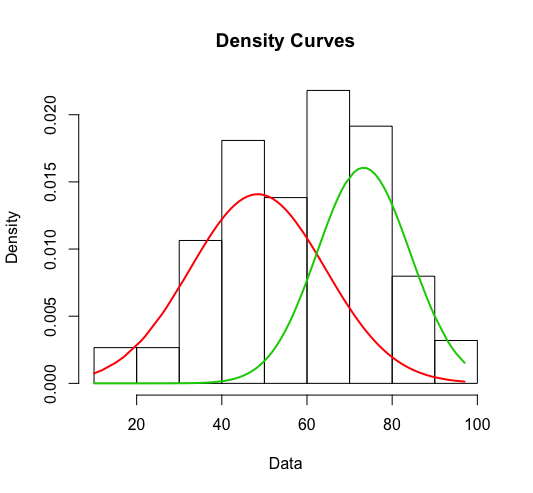
\includegraphics[width=\linewidth]{d1_intraPlot}
\end{figure}

\subsubsection*{Code R:}
\begin{verbatim}
> mean(intra$V1)
[1] 59.38298
> sd(intra$V1)
[1] 18.63388
>
>
> install.packages("flexmix")
> require("flexmix")
> kde <- density(intra$V1)ç
> m1 <- FLXMRglm(family = "gaussian")
> m2 <- FLXMRglm(family = "gaussian")
> fit <- flexmix(
    intra$V1 ~ 1,
    data = as.data.frame(intra$V1),
    k = 2,
    model = list(m1, m2))
> c1 <- parameters(fit, component=1)[[1]]
> c2 <- parameters(fit, component=2)[[1]]
> c1
Comp.1
coef.(Intercept) 72.28082
sigma            10.09489
> c2
Comp.2
coef.(Intercept) 41.31934
sigma            11.33671
>
>
> install.packages("mixtools")
> library(mixtools)
> intrab <- normalmixEM(intra$V1)
number of iterations= 386
> summary(intrab)
summary of normalmixEM object:
         comp 1   comp 2
lambda  0.55986  0.44014
mu     48.45378 73.28507
sigma  15.85827 10.93601
loglik at estimate:  -812.3421
> plot(intrab, which=2)
\end{verbatim}



\section{Baseball}
\subsection{Représentation arborescente dos-à-dos}
Il est possible en R de faire une représentation arborescente dos-à-dos avec l’extension \textit{aplpack} (Another Plot Package)\footnote{\url{https://stackoverflow.com/questions/25692421/how-do-you-make-a-comparative-stem-and-leaf-plot-in-r}}. On obtient le résultat suivant:
\begin{verbatim}
______________________
1 | 2: represents 0.12, leaf unit: 0.01 
    AL      NL  
______________________
      |  7 |9       
   981|  8 |69      
  7765|  9 |01377   
887631| 10 |00348   
     0| 11 |0       
     4| 12 |        
      | 13 |9       
______________________
n:    15      15  
______________________ 
\end{verbatim}

Par contre, il y a un problème au niveau de la valeur des feuilles. Au lieu de prendre la valeur arrondie, c’est la partie entière qui est prise. Ainsi, pour l’individu 29, les Yankees de New York en ligue américaine, le facteur du stade est à 0,816. Avec la virgule décimale un chiffre à gauche de la barre, le facteur du stade est noté 8|1 alors qu’il devrait noté 8|2, comme le fait par défaut la fonction stem.

En faisant la correction manuellement, on obtient :
\begin{verbatim}
______________________
  1 | 2: represents 0.12, leaf unit: 0.01 
      AL      NL  
______________________
      92|  8 |069      
   87750|  9 |12388   
  987632| 10 |00459  
       1| 11 |0       
       5| 12 |        
        | 13 |9       
______________________
n:    15      15  
______________________
\end{verbatim}
\subsubsection*{Code R:}
\begin{verbatim}
	> baseball<-read.table(file="~/d1_baseball.prn",header = TRUE)
> install.packages("aplpack")
> require("aplpack")
> AL <- baseball[baseball[,"Ligue"]=="AL","Points"]
> NL <- baseball[baseball[,"Ligue"]=="NL","Points"]
> stem(AL)
  The decimal point is 1 digit(s) to the left of the |

   8 | 29
   9 | 05778
  10 | 236789
  11 | 1
  12 | 5
> stem(NL)
  The decimal point is 1 digit(s) to the left of the |

   6 | 
   8 | 06912388
  10 | 004590
  12 | 9
> stem.leaf.backback(AL,NL,m=1,show.no.depths = TRUE)
\end{verbatim}


\subsection{Moyenne et écart-type}
La moyenne et l’écart-type ne sont pas des indicateurs robustes, ils sont sensibles aux valeurs extrêmes. Les deux groupes ont pratiquement la même moyenne (0,995 et 1,011), par contre, il y a une plus grande variation au niveau de l’écart-type : on a 0,106 pour la ligue américaine et 0,139 pour la ligue nationale. Soit une différence de plus de 30~\% ((0,139-0,106)/0,106). Y aurait-il des valeurs extrêmes dans le groupe de la ligue nationale?

\subsubsection*{Code R:}
\begin{verbatim}
> mean(AL)
[1] 1.011467
> mean(NL)
[1] 0.9952667
> sd(AL)
[1] 0.1060269
> sd(NL)
[1] 0.1389792
\end{verbatim}


\subsection{Valeur \og aberrante\fg{}}
Lors de la représentation dos-à-dos, si l’on avait laissé les paramètres par défaut, la valeur extrême aurait été plus facile visible (\texttt{HI: 1.394}) pour le groupe de la ligue nationale:
\begin{verbatim}
_____________________________
  1 | 2: represents 0.12, leaf unit: 0.01 
         AL       NL     
_____________________________
           |  7* |           
           |  7. |9      1   
   1      1|  8* |           
   3     98|  8. |69     3   
           |  9* |013    6   
   7   7765|  9. |77    (2)  
  (2)    31| 10* |0034   7   
   6   8876| 10. |8      3   
   2      0| 11* |0      2   
           | 11. |           
   1      4| 12* |           
           | 12. |           
           | 13* |           
_____________________________
                  HI: 1.394  
n:       15       15     
_____________________________
\end{verbatim}

Cette valeur est détectée comme aberrante selon la règle du 1,5 IQR. On le remarque tout de suite lorsque l’on fait un diagramme à moustaches, cf. fig.~\ref{baseballBoxplot}.

\begin{figure}[htbp]
	\caption{Valeur aberrante}
	\label{baseballBoxplot}
	\centering
	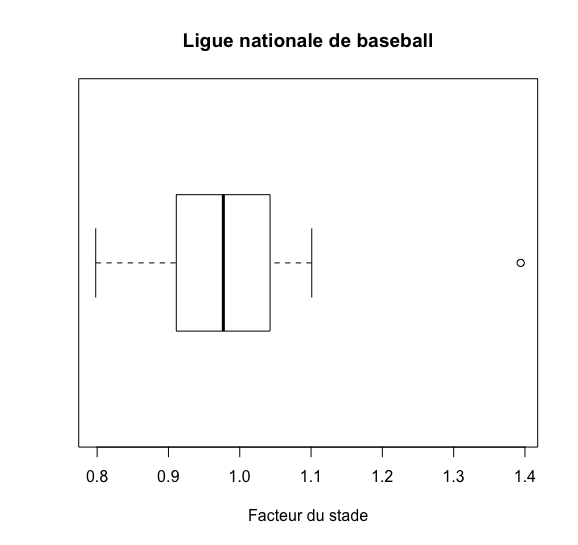
\includegraphics[width=\linewidth]{d1_baseballBoxplot}
\end{figure}

Lorsqu’on enlève la valeur considérée comme aberrante, la moyenne passe de 0,995 à 0,967 et l’écart-type de 0,139 à 0,088, ce qui fait une baisse de 37~\% de l’écart-type.

\subsubsection*{Code R:}
\begin{verbatim}
stem.leaf.backback(AL,NL)
boxplot(
  NL,
  main = "Ligue nationale de baseball",
  xlab = "Facteur du stade",
  horizontal = TRUE)
NL2 <- baseball[baseball[,"Points"]<="1.3"
  & baseball[,"Ligue"]=="NL","Points"]
> mean(NL)
[1] 0.9952667
> mean(NL2)
[1] 0.9667857
> sd(NL)
[1] 0.1389792
> sd(NL2)
[1] 0.08773577
\end{verbatim}



\section{Indice NASDAQ}
\subsection{Intervalle de confiance}
L’intervalle de confiance à 95~\% pour une loi $\mathcal{N}(\mu,\sigma) = \mathcal{N}(12,6 \%, 25,4\%)$ est $[-37,2 \%, 62,4 \%]$. À 95~\%, le retour annuel sur investissement sera entre -37,2 \% et 62,4 \%.

\subsubsection*{Code R:}
\begin{verbatim}
> round(qnorm(0.025, mean = 12.6, sd = 25.4), digits = 1)
[1] -37.2
> round(qnorm(0.025, mean = 12.6, sd = 25.4, lower.tail = FALSE),
    digits = 1)
[1] 62.4
\end{verbatim}


\subsection{Pourcentage d’année où le marché est baissier}
La probabilité d’avoir $X \leq 0$ pour une loi $\mathcal{N}(12,6 \%, 25,4\%)$ est de 30,7~\%. Le pourcentage d’année où le marché est baissier est de 30,7~\%.

\subsubsection*{Code R:}
\begin{verbatim}
> round(pnorm(0, mean = 12.6, sd = 25,4), digits = 3)
[1] 0.307
\end{verbatim}


\subsection{Pourcentage d’année où l’indice gagne plus de 25~\%}
La probabilité d’avoir $X \geq 25~\%$ pour une loi $\mathcal{N}(12,6 \%, 25,4\%)$ est de 31,0~\%. Le pourcentage d’année où l’indice gagne plus de 25~\% est de 31,0~\%.

\subsubsection*{Code R:}
\begin{verbatim}
> round(1 - pnorm(25, mean = 12.6, sd = 25,4), digits=3)
[1] 0.31
\end{verbatim}



\section{Wayne Gretzky}
\subsection{Histogramme}
L’histogramme du nombre de buts comptés par saison est représenté à la figure~\ref{gretzkyHist}.

\begin{figure}[htbp]
	\caption{Histogramme}
	\label{gretzkyHist}
	\centering
	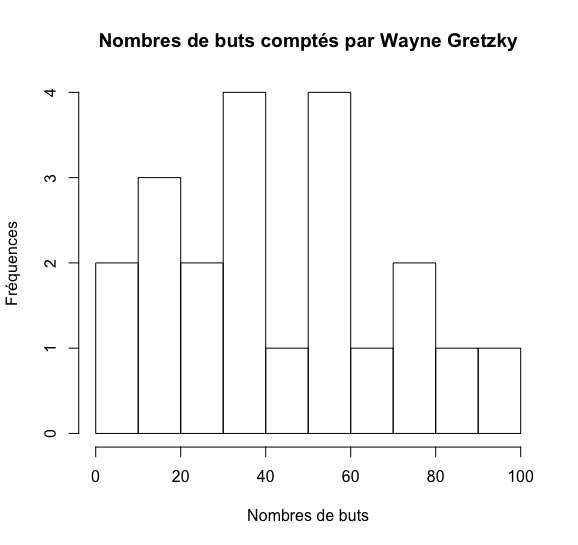
\includegraphics[width=\linewidth]{d1_gretzkyHist}
\end{figure}

\subsubsection*{Code R:}
\begin{verbatim}
gretzky<-read.table(file="~/d1_gretzky.txt")
hist(
  gretzky$V1,
  main = "Nombres de buts comptés par Wayne Gretzky",
  xlab = "Nombres de buts",
  ylab = "Fréquences")
\end{verbatim}


\subsection{Diagramme à moustaches}
Le diagramme à moustaches du nombre de buts comptés par saison est représenté à la figure~\ref{gretzkyBoxplot}.

\begin{figure}[htbp]
	\caption{Diagramme à moustaches}
	\label{gretzkyBoxplot}
	\centering
	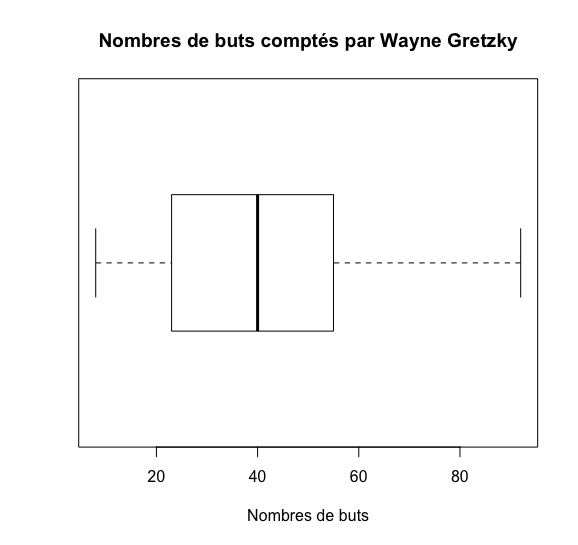
\includegraphics[width=\linewidth]{d1_gretzkyBoxplot}
\end{figure}

\subsubsection*{Code R:}
\begin{verbatim}
boxplot(gretzky$V1,
  main = "Nombres de buts comptés par Wayne Gretzky",
  xlab = "Nombres de buts",
  horizontal = TRUE)
\end{verbatim}


\subsection{Analyse succincte}
D’après l’analyse numérique, la moyenne étant plus grande que la médiane, la distribution serait légèrement asymétrique à droite. Ce qui se confirme avec le diagramme à moustache avec un quatrième quartile très étendu et également avec l’histogramme lorsqu’on compare l’intervalle~70-100 à l’intervalle~0-30.

\subsubsection*{Code R:}
\begin{verbatim}
> summary(gretzky$V1)
   Min. 1st Qu.  Median    Mean 3rd Qu.    Max. 
   8.00   23.00   40.00   42.57   55.00   92.00
\end{verbatim}


\subsection{Graphique temporelle}
En observant le graphique temporel (cf. fig.~\ref{gretzkyPlot}), on se rend compte que c’est la première moitié de la carrière qui est exceptionnelle. Il y aurait même une corrélation négative entre le nombre de buts par saison et les saisons. Pour cela, il suffit d’ajouter une variable pour la saisonnalité, afin de pouvoir calculer la corrélation. On obtient une corrélation négative de -0,85 entre les deux variables. Moralité : plus on gagne de l’expérience, moins on est bon!

\begin{figure}[htbp]
	\caption{Graphique temporelle}
	\label{gretzkyPlot}
	\centering
	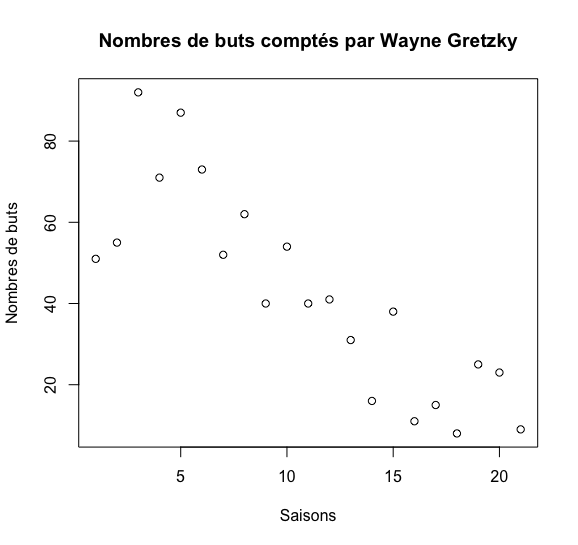
\includegraphics[width=\linewidth]{d1_gretzkyPlot}
\end{figure}

\subsubsection*{Code R:}
\begin{verbatim}
> plot(
    gretzky$V1,
    main = "Nombres de buts comptés par Wayne Gretzky",
    xlab = "Saisons",
    ylab = "Nombres de buts")
> gretzky$V2 <- seq(1,21)
> cor(gretzky$V1, gretzky$V2)
[1] -0.8507047
\end{verbatim}



\bibliographystyle{stat-fr}
\bibliography{STT1700}

\end{document}
